\begin{figure}[htbp]
\centering
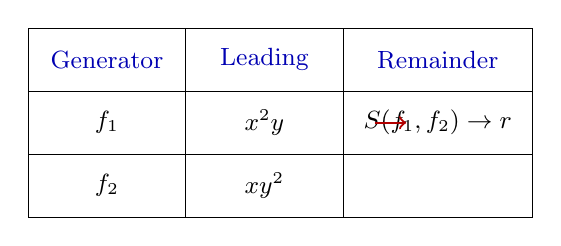
\begin{tikzpicture}[scale=0.8]
  \draw (0,0) rectangle (8,3);
  \draw (0,1)--(8,1);
  \draw (0,2)--(8,2);
  \draw (2.5,0)--(2.5,3);
  \draw (5,0)--(5,3);
  \node[font=\small,blue!70!black] at (1.25,2.5) {Generator};
  \node[font=\small,blue!70!black] at (3.75,2.5) {Leading};
  \node[font=\small,blue!70!black] at (6.5,2.5) {Remainder};
  \node[font=\small] at (1.25,1.5) {$f_1$};
  \node[font=\small] at (1.25,0.5) {$f_2$};
  \node[font=\small] at (3.75,1.5) {$x^2 y$};
  \node[font=\small] at (3.75,0.5) {$xy^2$};
  \node[font=\small] at (6.5,1.5) {$S(f_1,f_2) \to r$};
  \draw[->,thick,red!70!black] (5.5,1.5)--(6,1.5);
\end{tikzpicture}
\caption{Buchberger's algorithm: S-polynomials are formed from pairs of generators and reduced.}
\label{fig:grobner}
\end{figure}
